\documentclass{standalone}
\usepackage{tikz,tikz-3dplot}
\usetikzlibrary{perspective,patterns}
\usetikzlibrary{calc,fadings,decorations.pathreplacing}
\usetikzlibrary{shapes,fit}
\usetikzlibrary{hobby}
\usetikzlibrary{arrows.meta}
\begin{document}
\tikzset{illustration/.style={very thin}}
\tikzset{dimension/.style={very thin,lightgray}}
\begin{tikzpicture}[3d view={193.1664888870323}{-20.277404707870417},fill=gray]
\fill (0,-8.4)--(-8.4,0)--(0,8.4)--(8.4,0.0)--cycle;
\fill (5.25,0.0,152.4)--(0,5.25,152.4)--(-5.25,0,152.4)--(0,-5.25,152.4)--cycle;
\fill (0,-5.25,152.4)--(-5.25,0,152.4)--(0,5.25,152.4)--(5.25,0.0,152.4)--cycle;
\fill[white!8!black] (0.0,0.0,169.3)--(0,-5.25,152.4)--(5.25,0.0,152.4)--cycle;
\fill[white!54!black] (0.0,0.0,169.3)--(-5.25,0,152.4)--(0,-5.25,152.4)--cycle;
\fill[white!41!black] (0.0,0.0,169.3)--(5.25,0.0,152.4)--(0,5.25,152.4)--cycle;
\fill[white!80!black] (0.0,0.0,169.3)--(0,5.25,152.4)--(-5.25,0,152.4)--cycle;
\fill[white!13!black] (0,-8.4,0)--(5.25,0.0,152.4)--(0,-5.25,152.4)--cycle;
\fill[white!57!black] (-8.4,0,0)--(0,-5.25,152.4)--(-5.25,0,152.4)--cycle;
\fill[white!43!black] (8.4,0.0,0)--(0,5.25,152.4)--(5.25,0.0,152.4)--cycle;
\fill[white!86!black] (0,8.4,0)--(-5.25,0,152.4)--(0,5.25,152.4)--cycle;
\fill[white!57!black] (-8.4,0,0)--(0,-8.4,0)--(0,-5.25,152.4)--cycle;
\fill[white!13!black] (0,-8.4,0)--(8.4,0.0,0)--(5.25,0.0,152.4)--cycle;
\fill[white!86!black] (0,8.4,0)--(-8.4,0,0)--(-5.25,0,152.4)--cycle;
\fill[white!43!black] (8.4,0.0,0)--(0,8.4,0)--(0,5.25,152.4)--cycle;
\end{tikzpicture}
\end{document}
